\documentclass[letterpaper, titlepage]{article}

\usepackage[export]{adjustbox}
\usepackage{amsmath}
\usepackage[ngerman]{babel}
\usepackage[utf8]{inputenc}
% Tables
\usepackage{array}
\usepackage{graphicx}
\graphicspath{ {./Bilder/} }

\author{Simon Roske}
\title{Mathe Helfer}

\begin{document}
\maketitle

\tableofcontents
\listoffigures

\newpage

\newcommand{\skiptwolines}{
    \newline % Skip one line
    \newline % Skip another line
}

\newcommand{\skiptwolineswithcenteredexpr}[1]{
    \vspace{\baselineskip} % Skip one line
    \begin{center}
        #1 % Your centered expression goes here
    \end{center}
    \vspace{\baselineskip} % Skip another line
}

\newcommand{\absatzformel}{
    \hfill
    \break
}

\section{Zahlen}\label{Zahlen}


\subsection{Die natürlichen Zahlen $\mathsf{N}$}\label{Die natürlichen Zahlen}
Der Zahlenbereich der natürlichen Zahlen bildet das Zählen als natürlichen Prozess ab. Ob die 0 teil von $N$ ist, ist Definitionssache und nicht überall gleich. Angenommen, das sei nicht der Fall, dann gilt:
\skiptwolineswithcenteredexpr{$\mathsf{N}=\{1,2,3,4,…,n,n+1,…\}$.}
Wie kann man mit natürlichen Zahlen rechnen? Man darf uneingeschränkt addieren und multiplizieren. Man sagt $\mathsf{N}$ ist bezüglich der Addition und Multiplikation abgeschlossen. Alle anderen Rechenoperationen sind nicht uneingeschränkt durchführbar, da negative Zahlen nicht unter die Natürlichen fallen. Eine Untermenge von $N$ ist die Menge der \textbf{Primzahlen}, definiert als: 
\skiptwolineswithcenteredexpr{$\mathsf{P}=\{1,2,3,5,7,11,13,17,19,23,29,...\}$.}
Primzahlen sind nicht durch 1 und sich selbst teilbar!

\subsection{Die ganzen Zahlen $\mathsf{Z}$}\label{Die ganzen Zahlen}
Erweitert man den Zahlenbereich der natürlichen Zahlen mit negativen Zahlen, hat man die ganzen Zahlen: 
\skiptwolineswithcenteredexpr{$\mathsf{Z}=\{…-3,-2,-1,0,1,2,3,…\}$.}
Nun kann man auch uneingeschränkt subtrahieren.

\subsection{Rationale und irrationale Zahlen $\mathsf{Q}$, $\mathsf{R \backslash Q}$}\label{Rationale und irrationale Zahlen}
Will man uneingeschränkt dividieren, braucht man Bruchzahlen: 
\begin{itemize}
    \item $\mathsf{Q}_+$ enthält alle positiven Brüche: $\mathsf{Q}_+ = \{\frac{a}{b} \vert$ a,b sei eine natürliche Zahl und $b \neq 0\}$.
\end{itemize} 
Nimmt man negative Brüche dazu, hat man die rationalen Zahlen.
\begin{itemize}
    \item $\mathsf{Q} = \{\frac{a}{b} \vert$ a,b sei eine ganze Zahl und $b \neq 0\}$.
    \item In $\mathsf{Q}$ sind alle Grundrechenarten uneingeschränkt ausführbar.
    \item $\mathsf{Q}$ enthält alle positiven und negativen Brüche, sowie alle abbrechenden Dezimalbrüche \(z.B. -3,75-3,75\) und periodischen Dezimalbrüche (z.B. 0,66666…0,66666…).
\end{itemize}
Bei den rationalen Zahlen ist eines nicht vollständig erlaubt: Das Wurzelziehen, da es zu unendlichen Zahlen führt, die sich nicht als Bruch darstellen lassen, den \textbf{irrationalen Zahlen}: $\sqrt{2}=1,41421356..$. 

\subsection{Die reellen Zahlen $\mathsf{R}$}\label{Die reellen Zahlen}
Vereint man die rationalen und die irrationalen Zahlen, erhält man die reellen Zahlen $\mathsf{R}$. Jedoch: Wurzelziehen aus negativen Zahlen ist nicht definiert. Zum Beispiel ist $\sqrt{-4}$ nicht definiert. Solche Zahlen sind nicht in $\mathsf{R}$ enthalten.

\subsection{Komplexe Zahlen $\mathsf{C}$}\label{Komplexe Zahlen}
Eine komplexe Zahl - z - ist beschreibar als reelles Zahlenpaar: $x+iy|x,y \in \mathsf{R}, i = \sqrt{-1}$. Wichtig ist das mit der imaginären Zahl\ref{i - die imaginäre Zahl} das ziehen von negativen Wurzeln möglich ist. Man kann für c auch (x,y) schreiben, wobei x der Realteil und y der Imaginärteil ist. So kann die Menge der komplexen Zahlen ($\mathsf{C}$) auch in Form der reellen Zahlenpaare ($\mathsf{R}^2$) geometrisch auf der komplexen Ebene (auch Gaußsche Zahlenebene) dargestellt werden, siehe Bild unten.
\skiptwolines
Analog definiert man Addition wiefolgt: 
\\
\begin{align*}
    z_1 + z_2 &= (x_1 + x_2) + (y_1 + y_2)\cdot i \\
    z_1 - z_2 &= (x_1 - x_2) + (y_1 - y_2)\cdot i
\end{align*}
und Multiplikation so:
\\
\begin{align*}
    z_1 * z_2 &= (x_1 + x_2) * (y_1 - y_2)\cdot i = x_1 y_1 + x_1 y_2 \cdot i + y_1 x_2 \cdot i + x_2 y_2 \cdot i^2 \\
    z_1 * z_2 &= (x_y y_1 - x_2 y_2) + (x_1 y_2 + y_1 - x_2)\cdot i 
\end{align*}
\absatzformel
Ist $z$ eine komplexe Zahl, so ist $z^*$ die komplexe Konjugation. In der Darstellung unten würde der Realteil(z) hierbei gespiegelt. Als Spezialfall gilt: $i^* =-i$, sodass $z^* = x -y\cdot i$. Multipliziert mit dem komplexen Konjugat ergibt sich der Betrag von z. 
\skiptwolines
Den Betrag einer komplexen Zahl ergibt sich durch:
\skiptwolineswithcenteredexpr{$\vert z \vert = \sqrt{x^2+y^2}$}
Die Division ist definiert als: $\frac{z_1}{z_2} = \frac{z_1}{z_2} \cdot \frac{z_2*}{z_2*}$. Das ist nicht sehr angenehm und kann vermieden werden, wenn es nicht unbedingt sein muss. Sollte kein Weg daran vorbeiführen, so multipliere die Faktorden des Nenners und des Zählers je für sich und vereinfache so gut es gut mit der Definition von i.
\skiptwolines
Eine andere Darstellung ist mithilfe von Polarkoordinaten (\ref{Polarkoodinaten}) möglich:
\skiptwolineswithcenteredexpr{$z = a + i*b$  $\vert a, b, r \in \mathsf{R}, \theta \in [0,2\pi] \Leftrightarrow  z = r*(\cos(\theta)+i*\sin(\theta)) \Leftrightarrow r*e ^i\theta$.}

\subsection{Besondere Zahlen}\label{Besondere Zahlen}

\subsubsection{$\pi$ - Die Kreiszahl}\label{Die Kreiszahl}
3.1415926535\dots ..damit beginnt die irrationale Zahl $\pi$\footnote{8979323846 2643383279 5028841971 6939937510 5820974944 5923078164 0628620899 8628034825 3421170679 8214808651 3282306647 0938446095 5058223172 5359408128 4811174502 8410270193 8521105559 6446229489 5493038196 4428810975 6659334461 2847564823 3786783165 2712019091 4564856692 3460348610 4543266482 1339360726 0249141273 7245870066 0631558817 4881520920 9628292540 9171536436 7892590360 0113305305 4882046652 1384146951 9415116094 3305727036 5759591953 0921861173 8193261179 3105118548 0744623799 6274956735 1885752724 8912279381 8301194912}.Pi beschreibt das Verhältnis von Umfang zu Durchmesser eines Kreises. Es gibt viele Formeln, in denen $\pi$ die tragende Rolle spielt:


\begin{center}
\renewcommand{\arraystretch}{1.5} % Adjust the row height
\begin{tabular}{|c|}
\hline
Kreisumfang \\
\(U = \pi \cdot d = 2 \cdot \pi \cdot r\) \\
\hline
Kreisfläche \\
\(F = \pi \cdot r^2\) \\
\hline
Volumen \\
\(V = \frac{4}{3} \cdot \pi \cdot r^3\) \\
\hline
\end{tabular}
\renewcommand{\arraystretch}{1.0} % Reset the row height to default
\end{center}
\hfill

\subsubsection{$e$ - Euler's Zahl}\label{Euler's Zahl}
Die Eulersche Zahl ist die Basis des natürlichen Logarithmus, also $ln(e) = 1$. Die Eulersche Zahl kann beschrieben werden durch $e = 2,71828$..., aber ähnlich wie für $\pi$ gibt es keine exakte Lösung. Die Eulersche Zahl wurde nach dem Schweizer Mathematiker und Physiker Leonhard Euler \(1707-1783\) benannt. Unter anderem beinhaltet die natürliche Exponentialfunktion $f(x) = e^x$ die Eulersche Zahl. Für uns ist e vor allem wichtig, weil man anhand von der Eulerschen Formel $e^{j\phi}=\cos(\phi)+j*\sin(\phi)$ die komplexen Zahlen in der Exponentialform darstellen kann, was die Berechnungen erheblich erleichtert.

\absatzformel
Außerdem gilt $\partial e^t/\partial t=e^t$ was bedeutet, dass die Position von e gleich der Ableitung, also der Geschwindigkeitsänderung ist. Außerdem ist dieser Zusammenhang  besonders schön: 
\skiptwolineswithcenteredexpr{$\lim_{n \to \infty}\left(1+\frac{1}{n} \right)^n=2,718281828459...$} 
Damit is e der Grenzwert (\ref{Der Grenzwert}) der (exponentiell) steigenden Zahlenfolge.  

\subsubsection{i - die imaginäre Zahl}\label{i - die imaginäre Zahl}
\begin{center}
    
    $i^2=-1$
    \skiptwolines
    $i^3=-i$
    \skiptwolines
    $i^4=1$
    \skiptwolines
    $i^{-1}=-i$.
    \newline
\end{center}


\section{Grundlagen \& Rechengesetze}\label{Grundlegende Rechengesetze}
Eine Verknüpfung lässt sich definieren als die Art und Weise wie 2 Objekte ein Drittes definieren. Die Verknüpfung wird abstrakt mit '$\circ$' ausgedrückt.

\subsection{Kommutativgesetz}\label{Kommutativgesetz}
Die Reihenfolge der Verknüpfung spielt keine Rolle, e.g. $2\circ 3=3 \circ 2$. 

\subsection{Assoziativgesetz}\label{Assoziativgesetz}
Die Verknüpfung dreier Zahlen hängt nicht davon ab, wie wir sie gruppieren, e.g. $(2 \circ 3) \circ 4 = 2 \circ (3 \circ 4)$. 

\subsection{Distributivgesetz}\label{Distributivgesetz}
Der Umgang mit Klammern hängt vom Zahlenraum und der Art der Verknüpfung ab. Für Addition sowie Multiplikation für die Zahlenmenge $\mathsf{R}$ seien beide Verknüpfungen distributiv, sodass gilt: $2\odot (3\oplus 4)=2\odot 3\oplus 2\odot 4$. \hfill \break

\subsection{Die binomischen Formeln}
\begin{enumerate}
    \item[1]: $(a+b)^2=a^2+2ab+b^2$
    \item[2] $(a-b)^2=a^2-2ab+b^2$
    \item[3]  $(a+b)\cdot(a-b)=a^2-b^2$
\end{enumerate}

\subsection{Potenzen}\label{Potenzen}
Eine Potenz ist eine abgekürzte Schreibweise der Multiplikation.
\begin{itemize}
    \item $a^0=1$
    \item $a^1=a$
    \item $a^{-1}=\frac{1}{a}$ 
    \item $a^{-n}=\frac{1}{a^n}$
    \item $a^n=\frac{1}{a^{-n}}$
    \item $a^p * a^q = a^{p+q}$
    \item $a^p : a^q = a^{p-q}$
    \item $a^q * b^q = (a * b)^q$
    \item $a^q : b^q = (a : b)^q$
    \item $(a^p)^q = a^{p*q}$
    \item $\frac{a^m}{a^n}=a^{m-n}$
    \item $\frac{a^n}{b^n}=(\frac{a}{b})^n$.
    \item $(\frac{a}{b})^{-n}=(\frac{b}{a})^n$ 
\end{itemize}

\subsection{Wurzeln}\label{Wurzeln}
Die Wurzel einer Zahl ergibt mit sich selbst multipliziert die Wurzel. Im Normalfall handelt es sich um eine qudratische Multiplikation, aber auch höhere Wurzlen - e.g. die Kubische - ist denkbar. Als Potenz geschrieben ist die qudratische Wurzel $\sqrt{x}=x^{\frac{1}{2}}$ und $\sqrt[n]{x}=x^{\frac{1}{n}}$. Z.B.: $\sqrt[3]{125} = 125^{\frac{1}{3}}$.
Haben wir eine Potenz mit einer Lösung, dann gilt $x^n=a \Leftrightarrow x=\sqrt[n]{a}$.
\skiptwolines
Beispiel: $3^4 = 81 \equiv \sqrt[4]{81} = 3$
\skiptwolines
Randnotiz: Damit ist die n-te Wurzel die inverse Funktion (\ref{Inversibilität}) zu der Funktion: $x^n$, die abhängig von x ist (quadratische, kubische, etc.).

\subsection{Logarithmus}\label{Logarithmus}
\textbf{Frage}: Mit welcher Zahl muss ich a potenzieren um y zu bekommen? Geschrieben als $\log_a(x)=y$. Beachte, dass das Logarithmieren von Null und negativen Zahlen \textbf{nicht definiert} ist! 
\skiptwolines
Außerdem ist der Logarithmus die Umkehrfunktion zur Exponentialfunktion:
 
\skiptwolineswithcenteredexpr{$f(x)=a^x=y$, $f^{-1}(y)=\log_a(y)=x$} 
Also liefert der log. den Exponenten der Eexponentialfunktion zur Basis a. Haben wir die Exponentialfunktion $f(x)=e^x$ mit $e$ als Basis, so ist der Logarithmus Naturalis (ln) = $f^{-1}$. Der Logarithmus hat ein paar eigene Rechenregeln:\\
\begin{itemize}
    \item $\log_a(1)=0$
    \item $\log_a(a)=1$
    \item $\log_a(p*q)=\log_a(p)+\log_a(q)$
    \item $\log_a(\frac{p}{q})=\log_a(p)-\log_a(q)$
    \item $\log_a(p^q)=q*\log_a(p)$
    \item $\log_a(\sqrt[n]{p})=\frac{\log_a(p)}{n}$
    \item $\log_a(p)=\frac{\log_b(p)}{\log_b(a)}$
\end{itemize}
\vspace{0.6cm}
Logarithmische Skalierungen ist hilfreich, wenn die Daten stark variieren oder wenn die Verhältnisunterschiede zwischen Werten von Bedeutung sind, denn \textit{logarithmische Skalierung deckt einen größeren Bereich ab}. Beispiel:
\skiptwolines
$\log_{10}(10)=1, \log_{10}(100)=2, \log_{10}(1000)=3$.


\section{Geometrie}\label{Gemoetrie}


\subsection{Trignonometrie}\label{Trignonometrie}
Ein Einheitskreis ist definiert als ein Kreis mit radius 1. Das Interessante hierbei ist, dass sich die x- und y-Koordinate mithilfe von sinus und cosinus bestimmen lassen, abhängig vom Winkel. Man könnte auch sagen: 
\skiptwolineswithcenteredexpr{$\cos(\theta) = \frac{x}{1}$}
 und \skiptwolineswithcenteredexpr{$\sin(\theta) = \frac{y}{1}$}
 Ist der $radius \neq 1$ spielt der Wert r eine Rolle da die Division mit einem anderen Wert x und y verschiebt. Schließlich gilt auch für den radius (oder die Hypothenuse):
\skiptwolineswithcenteredexpr{$\tan(\theta) = \frac{y}{x}$.}
Die gewöhnliche Definition von sinus, cosinus und tangens, die sich auf Dreiecke bezieht, ist sehr ähnlich und hat demenstprechend Gemeinsamkeiten, die sich darin finden lassen, dass wir diese Dreicke einfach in den Einheitskreis einsetzen (siehe Abbildung \ref{Einheitskreis_Bild}).
\skiptwolines
\begin{align*}
    \sin(\theta) &= \frac{y}{z} = \frac{\text{Gegenkathete}}{\text{Hypothenuse}} \
    \\
    \cos(\theta) &= \frac{x}{z} = \frac{\text{Ankathete}}{\text{Hypothenuse}} \
    \\
    \tan(\theta) &= \frac{y}{x} = \frac{\text{Gegenkathete}}{\text{Ankathete}}
    \label{Trignonometrische Formeln}
    \end{align*}

 \begin{figure}[h]
    \begin{center}    
        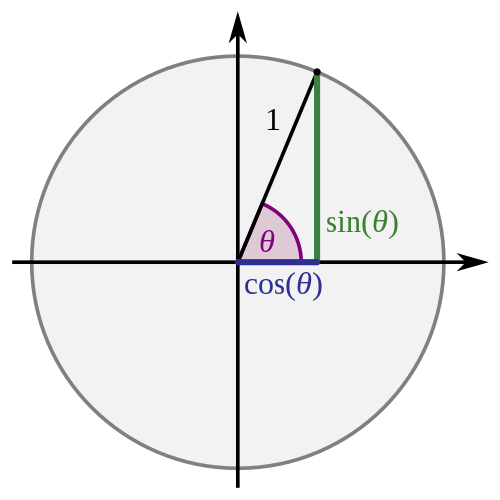
\includegraphics[scale=0.32]{Bilder/Sinus_und_Kosinus_am_Einheitskreis_1.svg.png}
        \caption[short]{Einheitskreis von der Wikipedia Seite. Vom 13. Oktober, 2023.}
    \end{center}
    \label{Einheitskreis_Bild}
\end{figure} \hfill \break
Fassen wir zusammen: Die expliziten Formeln zeigen, dass \textbf{Sinus}, \textbf{Cosinus} und \textbf{Tangens} einen Winkel nutzen um das Verhältnis zweier zueinander liegender Seite zu bestimmen. Da für den Einheitskreis der Divident = 1 ist, bilden sinus und cosinus so den x- und y-Wert ab, gegeben die X- und Y-Achse ist so orientiert. Dieses Bild reflektiert sehr schön, warum folgendes gilt:
\skiptwolines
\begin{align*}
    \sin(0) &= 0 \
    \\
    \cos(0) &= 1 \
    \\
    \sin(90) &= 1 \
    \\
    \cos(90) &= 0 \
    \\
    \sin(-\theta) &=  -\sin(\theta) \
    \\
    \cos(-\theta) &= \cos(\theta)
\end{align*}
Das ist auch der Grund, warum diese Funktionen (cos und sin) periodisch sind. Für Winkel $> 360$ kann man genauso gut Modulo rechnen und kommt wieder bei 0, bzw. 1 an.

\subsection{Polarkoodinaten}\label{Polarkoodinaten}
In Polarkoordinaten wird ein Punkt durch Angabe des Abstands r zum Koordinatenursprung und durch einen Winkel $\theta$ (auch Azimut genannt) bezüglich einer vorgegebenen Achse (z.B. der X-Achse) beschrieben. Das Zahlenpaar $(r,\theta)$ wird als Polarkoordinaten des Punktes bezeichnet. Umrechnen lassen sich die Koordinaten in das andere System wiefolgt:
\skiptwolines
Von Polarkoodinaten in kartesische Koordinaten:
\skiptwolineswithcenteredexpr{$x = r\cdot \cos(\theta)$ and $y = r\cdot \sin(\theta)$}
Von kartesischen Koordinaten in Polarkoordinaten:
\skiptwolines
Hier müssen wir zwei Dinge bestimmen. Der radius ist mittels Phytagoras gegeben, i.e. $r = \sqrt{x^2+y^2}$.  Ist der radius = 0, sind alle möglichen $\theta$ mögliche, daher gilt als (praktische) Lösung $\theta = 0$.
\skiptwolines
Außerdem sollte der der Wertebereichs des Winkels mit einem haloffenen Intervall gegeben sein, damit die Transformation eindeutig ist, i.e. $[0,2\pi)$. Der Winkel $\theta$ muss nach unterschiedlichen Fällen behandelt werden:    
\begin{align*}
        x > 0, y \geq 0: \theta = \arctan(\frac{y}{x}) \\
        \\
        x > 0, y < 0: \theta = \arctan(\frac{y}{x}) + 2 \pi \\
        \\
        x <0: \theta = \arctan(\frac{y}{x}) + \pi \\
        \\ 
        x = 0, y > 0: \theta = 90 \deg \\
        \\
        x = 0, y < 0: \theta = 270
        \\
\end{align*}
An dieser Stelle sei eine Besonderheit genannt. Wir wissen, dass für die Umrechnung $f_{P\rightarrow CK} = r*sin(\theta)=y, r*cos(\theta)=x$. Da sich r aus der Formel für den Tangens herauskürzen lässt, erhalten wir $tan(\theta)=\frac{\sin(\theta)}{\cos(\theta)}$. Anders formuliert beudetet das folgendes: Über den Winkel $\theta$ lässt sich mit $\tan(\theta)$ das Verhältnis $y:x$ berechnen. Daher können wir den Winkel $\theta$ mit der inversen zu berechenen. $f^{-1} \equiv \tan^{-1}(\frac{y}{x})$ übersetzt sich zu $\arctan(\frac{y}{x})$, woraus folgt: $\arctan(Gegenkahete/Ankathete)=\theta.\footnote{$\theta$ is in radian.}$
\skiptwolines
Werden Kreiskoordinaten mit einer dritten Koordinate ergänzt, ergeben sich räumliche Polarkoordinaten, wie z. B. Kugelkoordinaten oder Zylinderkoordinaten.
\subsubsection{Komplexe Zahlen mittels Polarkoodinaten}
$z \in \mathsf{C} = a + b\cdot i \equiv z = \vert z \vert \cdot e^{i\theta} = \vert z \vert (\cos(\theta) + i \cdot \sin(\theta)) = \vert z \vert \cdot \cos(\theta) + \vert z \vert \cdot i \cdot \sin(\theta)$

\subsection{Bogenmaß und Radian}\label{Bogenmaß und Radian}
Meistens werden Winkel in Grad angegeben. Aber ein Winkel von  bsp. 45 Grad kann auch in Bogenmaß ($\frac{1}{4}\pi \approx 0,79$) angegeben werden. Es gilt: $360\deg = 2\pi$, $1\pi = 180\deg$ und $1,5\pi = 270\deg$. Zu jedem Mittelpunktswinkel am Einheitskreis gehört ein Kreisbogen auf dem Einheitskreis. Die Länge des Kreisbogens ist ein Maß für die Größe des Winkels. Dieses wird als Bogenmaß bezeichnet und trägt die Einheit \textit{Radiant}, abgekürzt \textit{rad}. 
\begin{center}
    \framebox{$rad=\frac{\deg}{180\deg}*\pi$ und $\deg=\frac{rad}{\pi}*180\deg$}
\end{center}
\subsection{Phytagoras}\label{Phytagoras}
$a^2+b^2=c^2$


\section{Statistik}\label{Statistik}


\subsection{Statistische konzepte}\label{Statistische konzepte}

\subsubsection{Durchschnitt, modus, median}\label{Durchschnitt, modus, median}

\subsubsection{Varianz und Abweichung}\label{Varianz und Abweichung}

\subsubsection{Abhängige und unabhängige Variable}\label{Abhängige und unabhängige Variable}

\subsubsection{Korrelation}\label{Korrelation}

\subsection{Statistische verfahren}\label{Statistische verfahren}

\subsubsection{Pearson's chi-square test}\label{Pearson's chi-square test}


\section{Wahrscheinlichkeit}\label{Wahrscheinlichkeit}


\subsection{Kolmogorow' Axiome}\label{Kolmogorow's Axiome}
Kolmogorow's drei Axiome - so heißen die Grundsätze einer Theorie - sind die bekannteste Beschreibung der grundlegenden Eigenschaften der Wahrscheinlichkeitsrechnung. Seien $\Omega={\omega_1, \omega_2, \omega_3, \omega_4, \omega_5, \omega_6}$ die Ergebnismenge eines Zufallsexperiments, A und B Teilmengen von $\Omega$ und P eine Funktion, die jedem A eine reelle Zahl zwischen 0 und 1 zuordnet. P(A) wird Wahrscheinlichkeit genannt, falls folgende drei Bedingungen (Axiome) erfüllt werden:
\begin{enumerate}
    \item $P(A)\geq0$ Diese Bedingung besagt, dass jede Wahrscheinlichkeit für das Eintreffen einer Teilmenge von $\Omega$ (Ereignis) nicht negativ ist. Man nennt diese Eigenschaft daher auch: Nichtnegativität
    \item $P(\Omega)=1$ Das zweite Axiom bringt eine weitere Eingrenzung des Wertebereichs von der Funktion P. Mit Axiom 1 und 2 darf P(A) mit beliebigem A minimal Wert 0 und maximal Wert 1 annehmen.
    \item $P(A \cup B)=P(A)+P(B)$ Dies bedeutet also, dass für kein Ergebnis beide Ereignisse erfüllt werden. A und B nennt man in diesem Fall auch disjunkt.
\end{enumerate}

\subsection{Wahrscheinlichkeitskonzepte}\label{Wahrscheinlichkeitskonzepte}
Was ist gemeinsame, Grenz- und bedingte Wahrscheinlichkeit? Die Wahrscheinlichkeit gemeinsamer Erreignisse bedeutet, dass für die zwei Variablen ein Wert gegeben ist, also dass beispielsweise $P(X=male, Y=rugby)=\frac{100}{500}$. Man kommt auch zu diesem Ergebnis, indem man die bedingte Wahrscheinlichkeit mit der  Grenzwahrscheinlichkeit multipliziert, also $P(X,Y)=P(x)\cdot P(y|x)=P(y)\cdot P(x|y)=\frac{125}{500}\cdot \frac{100}{125}=\frac{270}{500}\cdot \frac{100}{270}$. Die  Grenzwahrscheinlichkeit ist die Wahrscheinlichkeit einer Kategorie anzugehören, also dass X=X und Y=y, oder andersherum. Ein Beispiel: $P(X=female)=\frac{230}{500}=0,46$ oder $P(Y=other)=\frac{180}{500}=0,36$. Schließlich die bedingte Wahrscheinlichkeit, also der Fall dass für eine Variable schon ein Wert gesetzt ist der den Wert der Zielvariable einschränkt bzw. spezifiziert, wir schreiben ganz generell: $P(X|Y)=\frac{P(X,Y)}{P(Y)}$.

\subsection{Wahrscheinlichkeitsverteilungen}\label{Wahrscheinlichkeitsverteilungen} Die Wahrscheinlichkeitsverteilung wird in zwei Arten unterteilt, die diskrete und die stetige Zufallsvariable. Diese sind dann jeweils noch mehrmals in verschiedene Kategorien unterteilt. Da es sich bei den Wahrscheinlichkeitsverteilungen um Funktionen handelt, gibt es immer einen Funktionswert und einen x-Wert.
Die \textbf{Diskrete Zufallsvariable} zeichnet sich dadurch aus, dass sie eine begrenzte, abzählbare Anzahl an möglichen Ausprägungen hat. Beispiele dafür sind der Münz- oder Würfelwurf. Beide haben nur eine begrenzte Anzahl an möglichen Ausprägungen, der Münzwurf hat zum Beispiel zwei und der Würfelwurf hat dafür 6 Ausprägungen. Die \textbf{kontinuierliche oder stetige Zufallsvariable} dagegen hat eine unbegrenzte Anzahl an möglichen Ausprägungen. Als Beispiel kann man dafür die Haarlänge nehmen. Theoretisch könnte man sagen, dass es von keinen Haaren, bis zu den weltweit längsten Haaren eine begrenzte Anzahl an Zentimetern gibt. Jedoch, wenn man die Länge in immer genaueren Einheiten angeben würdest, hätte man unendlich viele verschiedene Haarlängen auf der Welt, zumal es keine festgelegte Grenze für das Haarwachstum gibt. Die \textbf{Wahrscheinlichkeits Dichtefunktion} ist eine Wahrscheinlichkeitsfunktion, die kontinuierlich ist. Die Summe der Wahrscheinlichkeiten aller Ergebnisse ist in einem Zufallsexperiment immer gleich 1. In einer stetigen Zufallsverteilung muss die 1 auf unendlich viele Ausprägungen verteilt werden. Das führt dazu, dass die Wahrscheinlichkeit für eine einzelne Ausprägung praktisch gegen 0 geht. Ebendarum lässt sich in der Dichtefunktion nicht die Wahrscheinlichkeit einer einzelnen Ausprägung ableiten. Um aber trotzdem an ein Ergebnis zu gelangen, kannst du über mehrere Ausprägungen hinweg \textit{integrieren} und erhältst so die Wahrscheinlichkeit für diese Menge an Ausprägungen (Verteilungsfunktion). Genannt werden hier der Erwartungswert $E$, die Varianz $V$ (Standardabweichung ist $\sqrt V$), die Funktion der Wahrscheinlichkeitsverteilung, aber nicht die Verteilungsfunktion.

\subsubsection{Normalverteilung}\label{Normalverteilung}
Die Normalverteilung wird auch Gaußsche Glockenkurve genannt. Die beiden Parameter ($\mu$  und $\sigma$) geben Mittelwert sowie Standardabweichung der Normalverteilung an. Der zentrale Grenzwertsatz besagt, dass unter bestimmten allgemeinen Voraussetzungen die Summe aus n unabhängigen, identisch verteilten Zufallsvariablen wiederum normalverteilt ist. Als Beispiel se nehmen wir den Wurf von n fairen Würfeln: Wenn man man nur einen Würfel wirft, so ist jede Augenzahl gleich wahrscheinlich. Wirft man hingegen n-viele Würfel, so wird die mittlere Augenzahl durch die Normalverteilung beschrieben. Daher ist die Normalverteilung die Wichtigste, da natürliche Phänomene mit ausreichend großem n sich ihr annähern. Die Formel zur Berechnung der Verteilung lautet \textit{$f(x,\mu, \sigma)=\frac{1}{\sigma\sqrt{2\pi}}*e^{-\frac{1}{2}(\frac{x-\mu}{\sigma})^2}$}. Es gilt: $E=\mu$ und $V=\sigma^2$, bzw. $\sigma$ (Standardabweichung). Die gesamte Fläche, die von der Kurve der Normalverteilung eingeschlossen wird ist stets 1. Ist $\mu=0$ und $\sigma=1$ spricht man von der Standardnormalverteilung, die durch eine vereinfachte Gleichung (da $\mu=0$ wegfällt und $\sigma=1$) beschrieben wird: $\frac{1}{2\pi}e^-\frac{1}{2}x^2$. Der Vorfaktor stellt sicher, dass die gesamte Fläche unter der Kurve (und damit auch das Integral von -inf bis inf) eine Fläche von genau 1 hat. Die $\frac{1}{2}$ im Exponenten der e-Funktion gibt der Normalverteilung eine Einheitsvarianz. Jede Normalverteilung ist eine Variante der Standardnormalverteilung mit gestreckter Standardabweichung ($\frac{1}{\sigma}$) und \textit{z-transfomiertem} $\frac{x-\mu_x}{\sigma}$. Geschrieben wird die Normalverteilung für gewöhnlich so: $\mathcal{N}(\mu, \sigma^2)$. 

\subsubsection{Exponentialverteilung}\label{Exponentialverteilung}
Die Exponentialverteilung ist eine kontinuierliche Verteilung, die zur Modellierung der Dauer zufälliger Zeitintervalle genutzt wird. Der Parameter $\lambda$ steht für die Zahl der erwarteten \textit{Ereignisse} pro Zeitintervall. Als Beispiele nehmen wir hier die Länge eines Telefongesprächs oder der radioaktive Zerfall. Die Verteilung lässt keine negativen Werte zu, da negative Zeiten sinnlos sind. Sie wird in der Statistik häufig mit $\exp(\lambda)$ abgekürzt. Die Dichtefunktion ist folgendermaßen definiert:
\begin{flushleft}
        $f_{\lambda}(x) =
        \begin{cases}
            \lambda e^{-\lambda x} & \text{if } x \geq 0 \\
            0 & \text{if } x < 0 \\
        \end{cases}$.      
\end{flushleft} 
Der Erwartungswert $E$ ist defniert als $\frac{1}{\lambda}$, die Varianz $V$ als $\frac{1}{\lambda^2}$. Der Modus (der Wert, bei dem die Wahrscheinlichkeit am größten ist) liegt bei dieser Dichtefunktion bei $x_{mod}=0$. Möchte man die Wahrscheinlichkeit des Eintretens eines Ereignisses berechnen, so nutzt man dafür idealerweise die Verteilungsfunktion $F(x)$, die das Integral bis zu einem Wert x bildet. So entsteht eine akkumulierte Wahrscheinlichkeit $P(X\leq x)$.Oft ist die tatsächliche Verteilung keine Exponentialverteilung, jedoch ist die Exponentialverteilung einfach zu handhaben und wird zur Vereinfachung angewandt. Sie ist anwendbar, wenn ein Poisson-Prozess vorliegt, also die poissonschen Annahmen erfüllt sind. Die Exponentialverteilung ist ein Teil der viel größeren und allgemeineren Exponentialfamilie, einer Klasse von Wahrscheinlichkeitsmaßen, die sich durch eine leichte Handhabbarkeit auszeichnen.    

\subsubsection{Gleichverteilung}\label{Gleichverteilung}
Der französische Mathematiker Pierre Simon de Laplace (1749 bis 1827) untersuchte als einer der Ersten intensiv Zufallsexperimente, bei denen angenommen werden kann, dass jedes seiner Ergebnisse mit der gleichen Wahrscheinlichkeit eintritt. Zufallsexperimente mit Gleichverteilung heißen Laplace-Experimente. Die Gleichverteilung ist ein Sonderfall unter den Wahrscheinlichkeitsverteilungen, denn sie existiert sowohl als \textit{stetige} als auch als \textit{diskrete} Verteilung. Hier seien einmal kurz die Formeln für deren Berechnung genannt. Zuerst für den Fall einer diskreten Verteilung:
$f(x)=\frac{1}{n}, E(x)=\frac{n+1}{2}$ und $V(x)=\frac{1}{n}\sum_{0}^{n}(x_i-\mu)^2$. Und für eine stetige Verteilung: 
$f(x)=
\begin{cases}
    \frac{1}{b-a} & \text{if } a \leq x \leq b \\
    0 & \text{sonst} \\
\end{cases}$. a und b seien die Grenzen eines Intervalls, die x beinhalten. Da für alle x die gleiche Wahrscheinlichkeit gilt, ist diese von den Grenzen des Intervalls abhängig. $E(x)=\frac{a+b}{2} und V(x)=\frac{1}{12}\cdot (b-a)^2$.

\subsubsection{Poissonverteilung}\label{Poissonverteilung}
Die Poisson-Verteilung ist eine diskrete Wahrscheinlichkeitsverteilung, welche die Verteilung von Zählgrößen beschreibt. Oder mit anderen Worten: Wie oft tritt ein bestimmtes, zählbares Ereignis ein, wenn man es sehr oft wiederholt? Der Parameter gibt hierbei die mittlere Ereignisrate an.Die Wahrscheinlichkeit für die Zufallsvariable X der Poisson-Verteilung wird durch folgende Formel berechnet: $\frac{\lambda^x}{x!}\cdot e^{-\lambda}, x\in N_0$. Es besteht ein Zusammenhang zwischen Exponentialverteilung und Poissonverteilung. Beide betrachten denselben Sachverhalt aus verschiedenen Perspektiven. Die Exponentialverteilung gibt an, wie die Wahrscheinlichkeit der Dauer verschiedener Vorgänge verteilt ist. Die Poissonverteilung zählt, wie oft die gezählten Ereignisse in einem festgelegten Intervall auftreten. Ausgehend von der Exponentialverteilung soll ermittelt werden, wie die Wahrscheinlichkeit ist, dass genau n Ereignisse in einem Zeitintervall von t auftreten. Wie sich zeigen wird, ist das Ergebnis die Poissonverteilung. Da der Binomialkoeffiziert bei größeren Werten nur unter erhöhtem Rechenaufwand zu berechnen ist, kann man die Poisson-Verteilung benutzen, um die Binomialverteilung anzunähern. Man benutzt die Poisson-Verteilung im allgemeinen zu Annäherung der Binomialverteilung, wenn n groß ist und p klein. Als Erwartungswert $E=\mu$ der Poisson-Verteilung verwenden wir $\mu=\lambda=n \cdot p$, der mit der Varianz identisch istd. Allgemein approximiert die Poisson-Verteilung die Binomialverteilung sehr gut für Werte von $n \geq 100$ und $\lambda \leq 10$. Neben den Geschwindigkeitsvorteilen bei der Berechnung, hat die Poission-Verteilung noch den Vorteil, dass sie unendlich abzählbar ist, sich also ins positiv Unendliche inf fortsetzt.

\subsubsection{t-Verteilung oder Student-t-Verteilung}\label{t-Verteilung oder Student-t-Verteilung}
Die Normalverteilung wird bei vielen statistischen Verfahren eingesetzt. Allerdings unterschätzt die Normalverteilung bei kleinen Stichprobenumfängen die Standardabweichung. Dieser Effekt kann aber ausgeglichen werden, indem man bei manchen statischen Verfahren statt der Normalverteilung die t-Verteilung einsetzt. Die t-Verteilung ist eine der Normalverteilung verwandte Verteilung. Die t-Verteilung erhält man, wenn man den Mittelwert einer normalverteilten Population in Situationen schätzt, in denen der Stichprobenumfang klein\footnote{Eine gute Faustregel lautet, dass Sie bei einer Stichprobengröße von mindestens 30 die z-Verteilung anstelle einer t-Verteilung nutzen können.} ist und die Standardabweichung der Population unbekannt ist. Diese Verteilung zeichnet sich dadurch aus, dass Sie breitere Enden als die Normalverteilung hat. Für steigende Stichprobenumfänge nähern sich die beiden Verteilungen an und sind schließlich identisch. Die t-Verteilung ist folgendermaßen definiert: $T=\frac{Z}{\sqrt{\frac{1}{n}*\chi^2}}$, $E=0$ und $V=\frac{n}{n-2}$, wobei Z normalverteilt ist und $\chi^2$ unabhängig und \textit{$Chi^2$} verteilt ist.

\subsubsection{\textbf{$Chi^2$} Verteilung}\label{Chi Quadrat Verteilung}
Die $Chi^2$ Verteilung ist eine kontinuierliche Verteilung, die häufig zur Testung statistischer Unabhängigkeit oder zur Gültigkeit einer Hypothese (goodness of fit) genommen wird, genannt sei hier der \textit{Pearson's chi-square test}, \ref{Pearson's chi-square test}. Nur wenige weltliche Dinge sind mit der $Chi^2$ Verteilung gut beschrieben. Es gibt einen Parameter, der die Freiheitsgrade n festlegt\footnote{Würde man zufällige unabhängige Stichproben von n normalverteilten Größen nehmen, summierten sich diese Stichproben zu einer einer $Chi^2-V$ mit n Freiheitsgraden.}. Diese Freiheitsgraden bestimmen die Verteilung insofern, als dass $\chi_n^2=Z_1^2+...+Z_n^2$ gilt, also dass n unabhängige, quadrierte und standardnormalverteilte Zufallsvariablen ihr ungefähr äquivalent sind, d. h. $Z_k\sim \mathcal{N} (0,1) \forall k=1,...n$ und $\chi^2\sim\chi_n^2$. Außerdem gilt: $E_{Chi^2}=n$ und $V_{Chi^2}=2\cdot k$. 

\subsubsection{Binominalverteilung}\label{Binominalverteilung}
Prozesse bei denen nur 2 mögliche Ausgänge denkbar sind (e.g. ein Münzwurf) lassen sich mit der \textbf{Bi}nominalverteilung beschreiben. Voraussetzung dafür ist, dass das Experiment aus gleichen und von einander unabhängigen Versuchen besteht. Die Parameter n und k deuten schon darauf hin, dass es sich um eine diskrete Wahrscheinlichkeitsverteilung handelt, die Fragen nach k Erfolgen bei n Ereignissen beantwortet. Es gilt: 
\\
\begin{align}
    \begin{tabular}{|c|c|}
        \hline
        Variabel & Formel \\
        \hline
        $P(X=k)$ & $\binom{n}{k} \cdot p^k \cdot (1-p)^{n-k}$ \\
        $E$ & $n \cdot p$ \\
        $V$ & $n \cdot p \cdot q$ \\
        $\sigma$ & $\sqrt{n \cdot p \cdot q}$ \\
        $\binom{n}{k}$ & $\frac{n!}{k!(n-k)!}$ \\
        \hline
    \end{tabular}
\end{align}
\\
\\
Der Binominalkoeffizient beschreibt die Anzahl der Möglichkeiten, wie k Objekte in einer Gruppe aus n ohne Wiederholung angeordnet werden können. Die Binomialverteilung ist linksschief, wenn $p \geq 0,5$\footnote{Greather than aber nicht gleich! Symbol fehlt.}, rechtsschief wenn $p \leq 0,5$ und bei $p = 0,5$ symmetrisch. Wenn n hinreichend groß ist, kann die Normalverteilung als Annäherung zur Binomialverteilung verwendet werden, da die Schiefe mit zunehmenden n kleiner wird.

\subsubsection{Bernoulliverteilung}\label{Bernoulli}
Die Bernoulli Verteilung ist eine diskrete Verteilung, deren Zufallsvariable X nur zwei Werte annimmt: 0 = Misserfolg / Niete bzw. 1 = Erfolg / Treffer. Sie entsteht, wenn man ein Bernoulli Experiment (welches nur 2 mögliche Ausgänge hat) genau 1 Mal ausführt. Die Bernoulli Verteilung ist daher ein Spezialfall der Binomialverteilung für n=1. 
\\
Es gilt: $E_{bernoulli}=p, V_{bernoulli}=p\cdot (1-p)$ 
und $f_{bernoulli}(x)=\begin{cases}
    1-p & {if x=0} \\
    p & {if x=1} \\
    0 & {sonst.} \\
\end{cases}$

\subsection{Bayes}\label{Bayes}


\section{Algebra}\label{Algebra}
Ausgehend von dem Wissen was ein Vektor, ein Vektorraum und Basisvektoren sind, definieren wir eine lineare Transformation als eine Abbildung, welche den Nullvektor unverändert und die Linien aller Dimensionen im Vektorraum in den gleichen Abständen zueinander lässt\footnote[1]{Der Begriff der Linearität liegt hier vor.}. Für die Basisvektoren bedeutet dass, dass ein Vektor \textit{v}, für den gilt \textbf{Gl.1}: $v=3*\hat{i}+4*\hat{j}$ nach einer willkürlichen Transformation - wir können hier sagen nach Anwendung der Matrix \textit{A} auf \textit{v} - nach wie vor durch den Ausdruck \textbf{Gl.1} gegeben ist. Sei A eine quadratische Matrix in $R^n$, x und b Vektoren im selben Raum, dann ist A eine lineare Transformation auf x, geschrieben \textbf{Gl.2}: $A*x=b$. s
\\
\vspace{0.1cm}
\\
Im folgenden sind die 8 Axiome der Linearen Algebra:
\begin{enumerate}
    \item $u+(v+w)=(u+v)+w$
    \item $v+w=w+v$
    \item Es gibt den Nullvektor, sodass $v+0=v$
    \item Für jeden vektor v gibt es ein inverses, sodass gilt $v+(-v)=0$
    \item $a*(b*v)=(a*b)*v$
    \item $1*v=v$
    \item $a*(v+w)=a*v+a*w$
    \item $(a+b)*v=a*v+b*v$
\end{enumerate}


\subsection{Determinante}\label{Determinante}
Zur Veranschulichung empfiehlt es sich die $\det$ als Faktor vorzustellen, der Flächeninhalt/Volumen des Raumes, der von den Basisvektoren aufgespannt wird, skaliert. Ein Wert von Null bedeutet, dass der Raum in seinen Dimensionen reduziert wird und damit ist die Matrix weder invertierbar noch hat sie linear unabhängige Spalten. Gilt $\det(A)\neq0$, dann ist A invertierbar. Für \textbf{Gl.2} bedeutet das, dass $A^{-1}$ eine eindeutige Lösung besitzt. Ist $\det(A)\neq0$, so besitzt A entweder keine oder unendliche viele Lösungen.


\section{Analysis}\label{Analysis}


\subsection{Funktionen/Abbildungen}\label{Funktionen/Abbildungen}

\subsubsection{Definitionsbereich und Wertebereich}\label{Definitionsbereich und Wertebereich}
Die Definitionsmenge ist die Menge aller x-Werte, die in die Funktion eingesetzt werden dürfen. Die Wertemenge ist die Menge aller y-Werte, die die Funktion unter Beachtung ihrer Definitionsmenge annehmen kann. Wird jedes Element des Wertebereichs 'getroffen', so heißt die Funktion \textbf{surjektiv}. Bilden keine zwei Elemente des Definitionsbereichs auf dasselbe im Wertebereich ab, so heißt die Funktion \textbf{injektiv}. Ist eine Abbildung sowohl surjektiv als auch injekttiv, so heißt sie \textbf{bijektiv}.

\subsubsection{Spezielle Funktionen}\label{Die wichtigsten Funktionen}
Eine \textbf{lineare Funktion} ist einer Funktion der allgemeinen Form $f(x)=m\cdot x +b$.
\\ \\
\textbf{Quadratische} Funktionen haben die allgemeine Form $f(x)=a\cdot x^2+b\cdot x+c$. Dabei ist $a \neq 0$ und b und c Konstanten. Da $x^2$ der höchste Term ist (die höchste Ordnung) ist er der entscheidende Faktor für das Aussehen der Funktion\footnote{https://www.schlauerlernen.de/quadratische-funktion/}.
\\ \\
Eine Funktion $f$ mit der Funktionsgleichung $f(x)=x^n | n \in Z/\{0\}$ heißt \textbf{Potenzfunktion}. Wichtig ist hier zwischen den Exponenten zu unterscheinden, da hier grade/ungrade und positve/negative Exponenten die Potenzfunktion verschienden aussehen lassen. So nennt man Potenzfunktionen mit positivem Exponentem größer als 1 \textbf{Parabel}, und jene mit negativem Exponetem \textbf{Hyperbel}.
\\ \\
\textbf{Die Sigmoid Funktion}: Es gibt mehrere Sigmoidsche Funktionen. Zum Beispiel die \textbf{logistische Sigmoid}, \textbf{die Arctangent} und \textbf{die hyperbolische tangent Funktion}. Charakteristisch ist eine s-förmige Kurve, die du auch als logistische Kurve kennst. Sigmoidsche Funktionen mappen alle x-Werte zwischen 0 und 1 ($S_{log} \rightarrow$ Wahrscheinlichkeit), zwischen -1 und 1 ($S_{arctangent}$) oder noch größere Intervalle. Damit kann sie großartig als Aktivierungsfunktion in einem NN genutzt werden, um die letzte Schicht (output) zu erstellen. Außerdem ist bemerkenswert, dass die logistische Sigmoid für plus und minus unendlich gegen ihre spezifischen Limits covergiert. Daher hat sie stets Gradienten ungleich 0. Die \textbf{logistische Sigmoid} wird häufig nur \textbf{Sigmoid} genannt und wird so geschrieben:
\\ \\
$S(x)=\frac{1}{1+\exp(-x)} \equiv \frac{\exp(x)}{\exp(x)+1}$
\\ \\
Die \textbf{hyperbolische tangent Funktion}, die alle Werte in den Wertebereich = [-1,1] mapped, hat folgende Form:
\\ \\ $S_{tan}(x)=\frac{\exp(x)-\exp(-x)}{\exp(x)+\exp(-x)}$ 
\\ \\ 
Zuletzt genannt sei die \textbf{Arctangent Funktion}:
\\ \\
$S_{arc}(x)=arctan(x)$
\\ \\ 
Bekannt ist sie aus der Trignonometrie(\Ref{Trignonometrie}), da sie die inverse Funktion (\Ref{Inversibilität}) zur tangent Funktion ist. Ihr Wertebereich ist [$-2 \pi, 2 \pi$]. Die beiden letzteren Funktionen nähern sich viel schneller ihrem Grenzwert als für die klassische Sigmoid Funktion. Die \textbf{rectified linear Unit: ReLU} ist ebenfalls sehr bekannt aus KI. Sie wir geschrieben als: 
\\ \\
$ReLU(x)=max(0,x)$
\\ \\
Das coole an ihr, dass ihre Ableitung stets 1 ist für $x>0$ und dass sie nicht vom \textit{vanishing gradient} betroffen ist, der für große NN eine schnelle Konvergenz gegen 0 in der Backpropagation hat. In diesem Aspekt ist ReLU der Sigmoid klar überlegen, vorausgesetzt man kompensiert für negative x (deren Gradient $= 0$ ist), indem ein kleiner Term dazugerechnet wird.

\subsubsection{Inversibilität}\label{Inversibilität}
Eine Funktion heißt umkehrbar eindeutige (\textbf{eineindeutige}) Funktion, wenn nicht nur jedem Argument eindeutig ein Funktionswert zugeordnet ist, sondern auch umgekehrt zu jedem Funktionswert genau ein Argument gehört. Um die Umkehrfunktion einer Abbildung zu ehalten, löst man die Funktionsgleichung nach x um und vertauscht dann die Variablen. Zum Beispiel: $f(x)=x^2+1=y \rightarrow f^{-1}=x=\sqrt{y-1}$, vertauschen führt zu $f^{-1}=\sqrt{x-1}=y \hspace{0.1cm} | \hspace{0.1cm} \forall x \neq 1$. Allerdings, ist diese Funktion teilweise nicht definiert und daher nicht invertierbar. Das gilt nur solange wir die negativen Zahlen zulassen. Nehmen wir $\textit{R}^+$, ist $f(x)$ invertierbar.

\subsubsection{Nullstellen}
Nullstellen sind diejenigen Punkte einer Funktion, an denen der y-Wert den Wert 0 hat. Um sie auszurechnen setzen wir die Funktionsgleichung gleich 0 und lösen sie. Für Ableitungen ist das Verfahren dasselbe, doch hat es dann eine etwas andere Bedeutung, nämlich ist die (erste) Ableitung als Steigungsgraph der Funktion anzusehen, und diejenigen Punkte die im Ableitungsgraphen Nullstellen sind, sind in der \textbf{Stammfunktion} maxima oder minima. Die zweite Ableitung mit ihren Nullstellen gibt die \textbf{Wendepunkte} der Stammfunktion wieder. 

\subsection{Ableitungen}\label{Ableitungen}
Was beschreibt eine Ableitung? Die Ableitung beschreibt das Änderungsverhalten von Funktionen. Am interessantesten sind die erste und zweite Ableitung, da man hier graphisch leicht Nullstellen mit Maxima und Minima gleichsetzen kann. Die Nullstellen in der zweiten Ableitung geben Nullstellen der ersten Ableitung und damit Wende- oder Sattelpunkte der Abbildung wieder. Ableitungen werden mit $f'(x) = \frac{d f(x)}{dx} = \frac{d}{dx}f(x) = \frac{dy}{dx} = y'$ und mit $\partial$ für d (für partielle Ableitungen) kenntlichgemacht. 
\subsubsection{Spezielle Ableitungen}\label{Spezielle Ableitungen}
\begin{itemize}
    \item $f(x)=c \Rightarrow f'(x)=0$
    \item $f(x)=e^x \Rightarrow f'(x)=e^x$
    \item $f(x)=ln(x) \Rightarrow f'(x)=\frac{1}{x}$
    \item $f(x)=\sin(x) \Rightarrow f'(x)=\cos(x)$
    \item $f(x)=cos(x) \Rightarrow f'(x)=-\sin(x)$
    \item $f(x)=tan(x) \Rightarrow f'(x)=\frac{1}{cos^2(x)}$
\end{itemize}

\subsubsection{Ableitungsregeln}\label{Ableitungsregeln}
\begin{itemize}
    \item Potenzregel: $f(x)=x^n \Rightarrow f'(x)=n*x^{n-1}$
    \item Faktorregel: $f(x)=c*g(x) \Rightarrow f(x)=c*g'(x)$
    \item Summenregel/Differenzregel: $f(x)=h(x)+g(x) \Rightarrow f'(x)=h'(x)+g'(x)$
    \item Produktregel: $f(x)=h(x)*g(x) \Rightarrow f'(x)=h'(x)*g(x)+h(x)*g'(x)$
    \item Kettenregel: $f(x)=h(g(x)) \Rightarrow f'(x)=h'(g(x))*g'(x)$
    \item Quotientenregel: $f(x)=\frac{g(x)}{h(x)} \Rightarrow f'(x)=\frac{g'(x)*h(x)-g(x)*h'(x)}{h(x)^2} $
    \item Linearität: $f'(a*x)=a*f'(x)$ und $f'(x+z)=f'(x)*f'(z)$
\end{itemize}

\subsubsection{Partielle Ableitungen $\partial$}\label{Partielle Ableitungen}
Die Ableitung einer Funktion mit mehreren Argumenten nach einem dieser Argumente heißt partielle Ableitung. Das Argument, nach dem nicht abgeleitet wird, verhält sich wie eine Konstante.\hfill\break
\\\setlength{\fboxrule}{1pt} % Frame thickness
\framebox{$f_x=\frac{\partial f}{\partial x}$, $f_y=\frac{\partial f}{\partial y}$, $f_{xy}=\frac{\partial^2 f}{\partial xy}$, $f_{x}=\frac{\partial^2 f}{\partial x}$, $f_{yx}=\frac{\partial^2 f}{\partial yx}$}

\subsection{Polynome}\label{Polynome}

\subsection{Integrale}\label{Integrale}

\subsection{Der Grenzwert}\label{Der Grenzwert}

\subsection{Differentialgleichungen}\label{Differentialgleichung}
Eine Differentialgleichung ist eine Gleichung, in der eine Funktion und auch Ableitungen von dieser Funktion auftauchen können. Die Lösung dieser Art von Gleichung ist eine \textbf{Funktion, keine Zahl}! Die explizite Darstellung einer DGL erhalten wir, wenn wir die DGL auf die höchste vorkommende Ableitung umstellen können. Falls das nicht möglich ist, kann die DGL nur in impliziter Darstellung geschrieben werden. Also explizit: y\'= Ausdruck, implizit: Audruck + y\' = Ausdruck. Wir unterscheiden zwischen gewöhnlichen DGL, bei denen die gesuchte Funktion von einer Variable abhängt, bzw. es tauchen nur Ableitungen nach einer Variablen auf, und die partielle DGL. Hier hängt die gesuchte Funktion von mehreren Variablen ab und es tauchen partielle Ableitungen der Funktion auf. Die Ordnung einer DGL ist stets n, die höchste enthaltene Ableitung. Alle anderen Ableitungen niedrigerer Ordnung sind Funktionsargumente. Außerdem unterscheidet man zwischen linearen und nicht-linearen DGL, wobei erstere als Linearkombination explizit geschrieben werden kann, $y^n+a_{n-1}(x)y^{n-1}+...+a_2(x)y^2+a_1(x)y=b(x)$. Ist das nicht der Fall, ist die DGL nicht-linear. In vielen Büchern und Skripten taucht die Typisierung autonome DGL auf. Eine DGL heißt autonom, wenn die Variable x nicht explizit in der DGL auftaucht (also lediglich versteckt als Funktionsargument in der Funktion y und deren Ableitungen).
\begin{enumerate}
    \item 
\end{enumerate}

\subsection{Divergenz}\label{Divergenz}

\subsubsection{Kullback-Leibler}\label{Kullback-Leibler}
$D_{KL}=\mathbf{E}=[log(\frac{p(x)}{q(x)} )]= \int_{a}^{b}  \log (p(x)/q(x))\,dx  $

\subsubsection{Jensen-Shannon}\label{Jensen-Shannon}


\subsection{Lösungstrategien}
Wir beschreiben hier ein paar generelle Technicken und Tricks, die beim Lösen von Gleichungen hilfreich sein können. 
\begin{enumerate}
    \item Binomische Formeln nutzen 
    \item Faktorisieren: $2x^3+4x^2-2x-4=0 \equiv 2(x+1)(x-1)(x+2)$
\end{enumerate}


\subsection{Regression}\label{Regression}

\subsubsection{Lineare Regression}\label{Lineare Regression}

\subsubsection{Polynomilae Regression}\label{Polynomilae Regression}

\subsubsection{Logistische Regression}\label{Logistische Regression}


\section{Modellierung}


\end{document}